\documentclass[tikz,border=10pt]{standalone}
\usepackage{amsmath}
\begin{document}
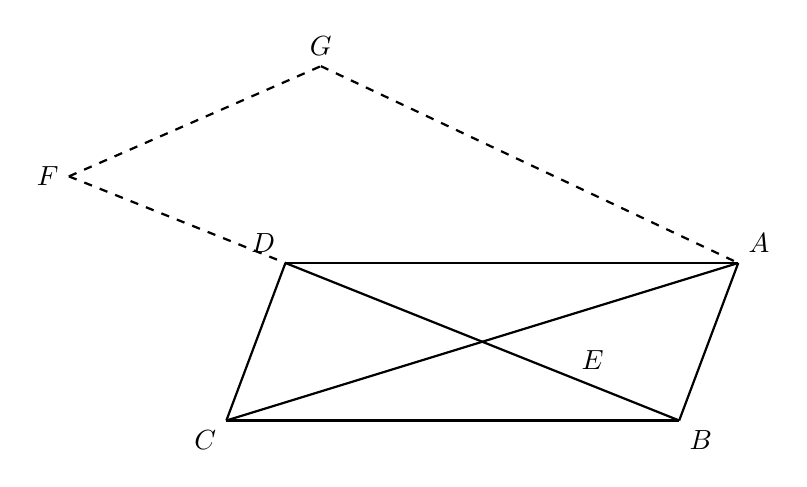
\begin{tikzpicture}[thick, scale=0.05]
  % Points (chosen coordinates approximating the figure)
  \coordinate (A) at (100,0);
  \coordinate (B) at (85,-40);
  \coordinate (C) at (-30,-40);
  \coordinate (D) at (-15,0);
  \coordinate (E) at (63,-19.5);
  \coordinate (F) at (-70,22);
  \coordinate (G) at (-6,50);

  % Solid edges
  \draw (D) -- (A);
  \draw (A) -- (B);
  \draw (B) -- (C);
  \draw (C) -- (D);
  \draw (C) -- (A);
  \draw (D) -- (B);

  % Dashed edges
  \draw[dashed] (F) -- (D);
  \draw[dashed] (F) -- (G);
  \draw[dashed] (G) -- (A);

  % Labels
  \node[above left] at (D) {$D$};
  \node[above right] at (A) {$A$};
  \node[below right] at (B) {$B$};
  \node[below left] at (C) {$C$};
  \node[below] at (E) {$E$};
  \node[left] at (F) {$F$};
  \node[above] at (G) {$G$};
\end{tikzpicture}
\end{document}
